%% ****** Start of file apstemplate.tex ****** %
%%
%%
%%   This file is part of the APS files in the REVTeX 4 distribution.
%%   Version 4.1r of REVTeX, August 2010
%%
%%
%%   Copyright (c) 2001, 2009, 2010 The American Physical Society.
%%
%%   See the REVTeX 4 README file for restrictions and more information.
%%
%
% This is a template for producing manuscripts for use with REVTEX 4.0
% Copy this file to another name and then work on that file.
% That way, you always have this original template file to use.
%
% Group addresses by affiliation; use superscriptaddress for long
% author lists, or if there are many overlapping affiliations.
% For Phys. Rev. appearance, change preprint to twocolumn.
% Choose pra, prb, prc, prd, pre, prl, prstab, prstper, or rmp for journal
%  Add 'draft' option to mark overfull boxes with black boxes
%  Add 'showpacs' option to make PACS codes appear
%  Add 'showkeys' option to make keywords appear
%\documentclass[aps,prl,preprint,groupedaddress]{revtex4-1}
%\documentclass[aps,prl,preprint,superscriptaddress]{revtex4-1}
\documentclass[aps,prl,reprint,groupedaddress,amsmath,amssymb,aps]{revtex4-1}

% You should use BibTeX and apsrev.bst for references
% Choosing a journal automatically selects the correct APS
% BibTeX style file (bst file), so only uncomment the line
% below if necessary.
%\bibliographystyle{apsrev4-1}

\usepackage{graphicx}% Include figure files
\usepackage{dcolumn}% Align table columns on decimal point
\usepackage{bm}% bold math

\begin{document}
	
	
	% Use the \preprint command to place your local institutional report
	% number in the upper righthand corner of the title page in preprint mode.
	% Multiple \preprint commands are allowed.
	% Use the 'preprintnumbers' class option to override journal defaults
	% to display numbers if necessary
	%\preprint{}
	
	%Title of paper
	\title{Laser Attenuation through Dyed Solution}
	
	% repeat the \author .. \affiliation  etc. as needed
	% \email, \thanks, \homepage, \altaffiliation all apply to the current
	% author. Explanatory text should go in the []'s, actual e-mail
	% address or url should go in the {}'s for \email and \homepage.
	% Please use the appropriate macro foreach each type of information
	
	% \affiliation command applies to all authors since the last
	% \affiliation command. The \affiliation command should follow the
	% other information
	% \affiliation can be followed by \email, \homepage, \thanks as well.
	\author{Jacob Miller}
	%\email[]{Your e-mail address}
	%\homepage[]{Your web page}
	%\thanks{}
	%\altaffiliation{}
	\affiliation{UCSB CCS Physics}
	
	%Collaboration name if desired (requires use of superscriptaddress
	%option in \documentclass). \noaffiliation is required (may also be
	%used with the \author command).
	%\collaboration can be followed by \email, \homepage, \thanks as well.
	%\collaboration{}
	%\noaffiliation
	
	\date{\today}
	
	\begin{abstract}
	After light travels through an opaque solution it appears dimmer. The effect that solutions have on light can be studied precisely by measuring the intensity of a laser beam after it passes through a cell containing diluted dye. As the beam of light travels through the solution, it encounters and interacts with particles of dye. We expect that the presence of these particles will cause an attenuation in the power of the light beam. By comparing the power of light transmitted through a solution to the power of the unimpeded laser, we discover the effect that varying solutions have on a beam of light.
	\end{abstract}
	
	% insert suggested PACS numbers in braces on next line
	\pacs{}
	% insert suggested keywords - APS authors don't need to do this
	%\keywords{}
	
	%\maketitle must follow title, authors, abstract, \pacs, and \keywords
	\maketitle
	
	% body of paper here - Use proper section commands
	% References should be done using the \cite, \ref, and \label commands

	\section{\label{sec:level1}Introduction}
	Intuition tells us that when light shines through an opaque fluid it appears dimmer on the opposite side. Imagine trying to find the keys you dropped in a pond with clear water versus one with murky water. The image of the bottom of the pond is dimmer in the murky water. 
	
	This phenomenon occurs because the murky water contains suspended particles which can impede the path of a photon. To investigate this effect, we will measure the attenuation of a light as it passes through a cell containing dyed liquid. The results will help build a precise relationship between the properties of a fluid and the attenuation of a beam of light that travels through it.
	
	Results of this experiment will allow us to predict the transmission of light through any fluid. A mathematical model of the attenuation of light through a fluid can be applied in various fields of science. For instance, communication by submarines and by satellites both rely on sending information
	
	\section{Theory}
	Light traveling through a dyed fluid is impeded by the particles suspended in that fluid. A photon that travels through a solution of greater concentration has a better chance of encountering a particle, as does a photon that travels a greater distance through a solution.
	
	We suspect that the attenuation of a beam passing through a dyed fluid is dependent on the chance of each photon encountering a suspended particle. Clearly, this chance increases as the number of particles in the photon's path increases. Considering the beam of light as a whole, the total attenuation should depend on the number of suspended dye particles in the beam's path.
	
	To calculate the number of particles in the path of the beam, we first consider in Fig~\ref{laservolume} the cylindrical volume of fluid that the laser will interact with. 
	\begin{figure}
		\includegraphics{fig_1}
		\caption{\label{laservolume}}
	\end{figure}
	The volume of this region is described by
	\begin{equation}
		V=2\pi r_L^2 \cdot d
	\end{equation}
	where $r_L$ is the radius of the laser beam and $d$ is the length of the cell.
	
	If we define the concentration of the fluid $C$ by Eqn~\ref{conc}, we can calculate the number of particles in the beams path $N_p$ as shown in Eqn~\ref{Npath}.
	\begin{equation}
	\label{conc}
	C = n \frac{1}{[V]}
	\end{equation}
	\begin{equation}
		\label{Npath}
		N_p = V\cdot C = 2\pi r_L^2 \cdot d \cdot C
	\end{equation}
	
	Notice in equation~\ref{Npath} that $r_L$ is fixed so $N_P$ only depends on $d\cdot C$. For this reason, we design our procedure to control the length of the cell and the concentration of the dyed fluid to produce varying values of $N_P$.
	
	\section{\label{sec:level1}Experimental Methods}
	In this paper we study the effect that a dyed fluid has on a beam of light by varying the concentration of the dye and the distance the beam travels through it. Light is provided by a 12mW laser producing a red beam.
	
	\subsection{Varying Distance Laser Travels through Solution}
	To vary length of the solution we use machined cells of varying lengths as illustrated in Fig~\ref{cellDiagram}.
	\begin{figure}[b]
		\includegraphics{fig_1}
		\caption{\label{cellDiagram}The 10cm cell}
	\end{figure}
	The cells are constructed with a metal base, plastic siding, and glass windows on either end. The pieces are glued together. We vary the length of the cell to change the distance the laser travels the solution, in turn varying $N_p$.
	
	\subsection{Varying Concentration of Blue Dye Solution}
	To vary the concentration of the solution we perform dilutions of a stock blue dye. Dilutions are carried out by measuring a volume of stock solution in a graduated cylinder, adding it to the empty 10cm cell, and then adding a volume of water as measured in a graduated cylinder.
	
	Starting with the base solution of 1.00 concentration, half dilutions are performed by adding 18ml of the current solution to 18ml of water. According to Eqn~\ref{dilutioneq},
	\begin{equation}
		\label{dilutioneq}
		V_1 \cdot C_1 = V_2 \cdot C_2
	\end{equation}
	starting with 18ml and ending with 36ml, our concentration should reduce by a factor of 2. 
	
	Performing dilutions in this way means that we will always have 36ml of each solution which is sufficient to almost fill up the largest cell (Fig~\ref{cellDiagram}) which has volume given by Eqn~\ref{v10cell}.
	\begin{equation}
		\label{v10cell}
		L \cdot W \cdot H=10\mathrm{cm}\cdot 1.5\mathrm{cm}\cdot 2.5\mathrm{cm}=37.5\mathrm{cm}^3=37.5\mathrm{ml}
	\end{equation}
	Smaller cells can be filled by transferring the solution from the previous cell after it has been tested. In this way we can ensure that solution is identical for each cell.
	
	\subsection{Distances in Setup}
	The measurement procedure consists of placing the cell on a platform between a laser and the detector that are mounted on a metal track that is about $35cm$ long. The laser, platform, and detector are all free to slide along the track and in this way the distances between the components can be adjusted.
	
	The front face of the cell is always positioned 18cm from the laser and the distance between the laser and the detector is kept fixed at 30cm as illustrated in Fig~\ref{setup}.
	\begin{figure*}
		\includegraphics{fig_2}
		\caption{\label{setup}The alignment of the laser, cell, and detector}
	\end{figure*}

	The setup is intended to maximize the distance between the laser source and the cell because, as supported by Fig~\ref{distancetest},
	\begin{figure}[b]
		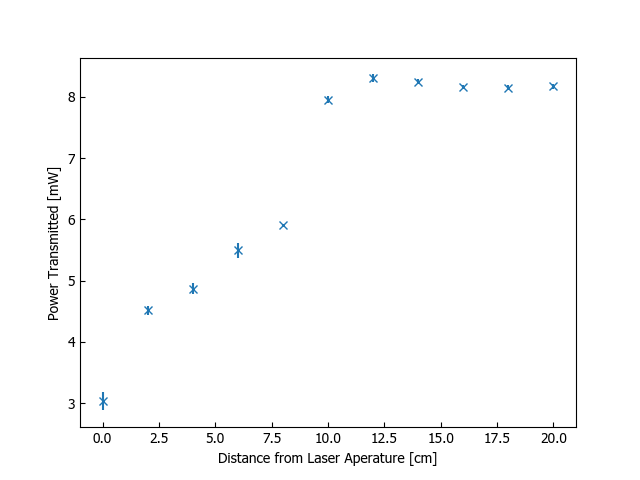
\includegraphics[width=\columnwidth]{distTest.png}
		\caption{\label{distancetest}Power transmitted by laser through an empty cell at varying distances from the laser}
	\end{figure}
	a greater separation reduces the contribution of factors other than cell length and solution concentration. We suspect that placing the cell close to the window increases the amount of light that is reflected back into the laser source, which in turn affects our measurements.
	
	\subsection{Angle of Incidence}
	To ensure that there is little variation in the angle of incidence of the laser upon the cell, we align each cell against the laser housing before sliding it in to position along the rail. In this way the angle of incidence will not only be consistent between cells and trials, but the cell windows will also be aligned nearly perpendicular to the incident laser beam.
	
	\subsection{Readout}
	To read out the intensity of the laser we used an electronic power scale in conjunction with a digital multimeter. The scale was zeroed to the ambient light of the room before every use. The scale was also set to read 20mW max power. The output on the multimeter ranged from 0mV to 500mV regardless of the range of the scale. This allows power to be calculated from multimeter readout using Eqn~\ref{readout}.
	\begin{equation}
		\label{readout}
		P [\mathrm{mW}] =\frac{V [\mathrm{mV}]}{500 \mathrm{mV}} * 20 \mathrm{mW}
	\end{equation}	
	
	\subsection{Trials}
	A trial consists of testing a certain concentration in a certain size cell. Trials were grouped by concentration value, and an addition trial was added at the beginning of each group to measure the intensity of the unimpeded laser.
	
	Before each individual trial, the laser is switched off for at least 10 seconds. During this time the cell is aligned between the laser and the detector. When the laser is turned on, there is a 10 second period where no readout is performed. This is to allow the power to stabilize. After this 10 second period, the detector readout is monitored for 120 seconds during which time the maximum and minimum readout values are recorded.
	
	\section{\label{sec:level1}Results}
	Figure~\ref{trans}
	\begin{figure}
		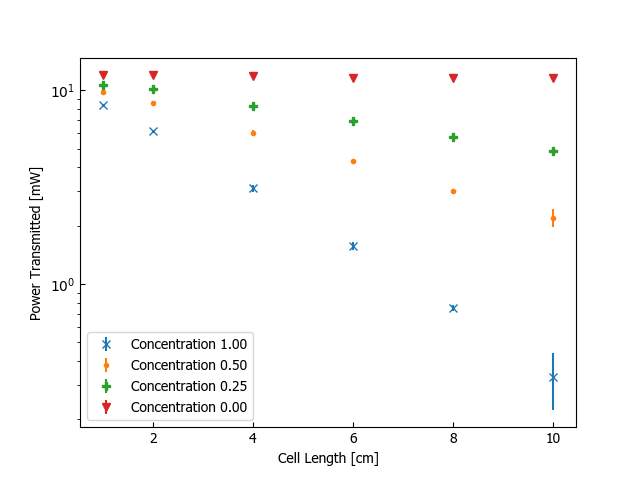
\includegraphics[width=\columnwidth]{trans.png}
		\caption{\label{trans}Power transmitted through varying cell sizes with concentration of 1.00, 0.50, 0.25, and 0.00 units. Plotted on a logarithmically scaled y-axis}
	\end{figure}
	shows the results of changing cell length for each concentration on a logarithmically-scaled y-axis. The linear trend of each set of points on this plot that appears when scaled as such suggests that the relationship can be modeled using a power function for each cell length. It is important to note that each line approaches near to the same y-intercept. This is an expected result considering concentration of the fluid should have no effect as length approaches $0$.
	
	When studying the power transmitted through the solution it is more useful to compare the transmitted power to the unimpeded power of the laser. Figure~\ref{transRatio}
	\begin{figure}
		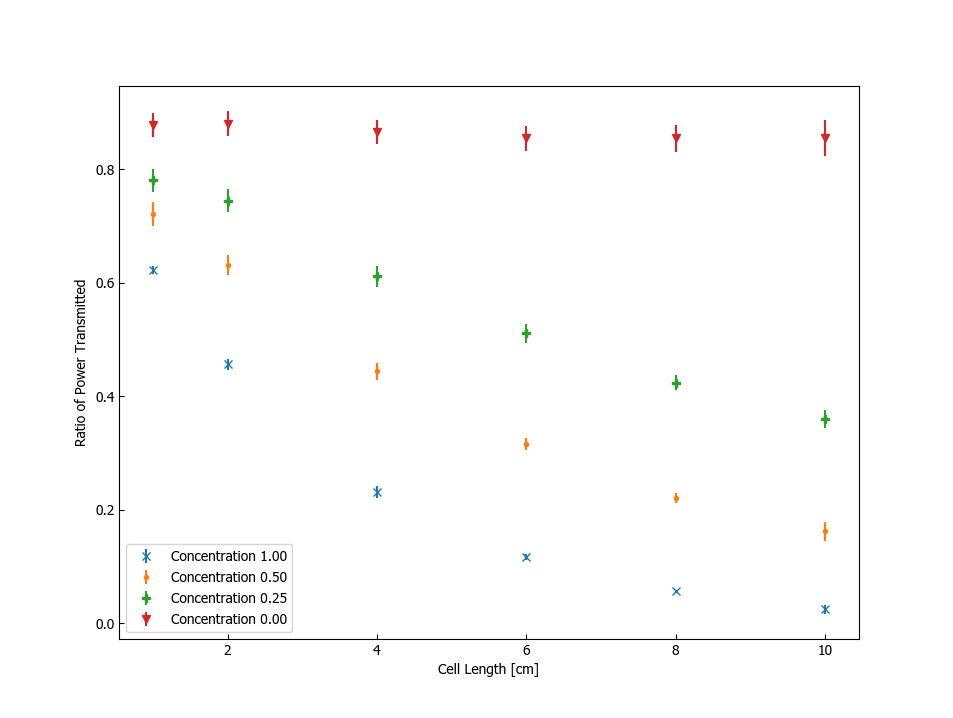
\includegraphics[width=\columnwidth]{transRatio.png}
		\caption{\label{transRatio}Ratio of power of laser that is transmitted through the solution}
	\end{figure}
	shows a plot of these ratios.
	
	\section{\label{sec:level1}Analysis}
	In addition to the effect of the solution on the power of the beam, we must also consider the consequences of the beam traveling through the two glass plates that contain the solution.
	
	We know that light is reflected at a boundary between two materials causing a decrease in power according to
	\begin{equation}
		P_T = T_b*P_0
	\end{equation}
	where $T_b$ is a constant coefficient which is a property of the specific boundary. We also know that $T_b$ does not depend on which direction the light crosses the boundary.
	
	In our experiment we assume that $T_b$ on the boundary of glass and any concentration of solution is the same as $T_b$ on the boundary of glass and water.
	
	In order to account for the effect of light going through two glass panes before incidence upon the detector, we must know $T_b$ for the air-glass boundary ($T_1$) and for the glass-water boundary ($T_2$).
	
	If the power transmitted by the laser through the solution without the glass panes is a function
	\begin{equation}
		P = P(P_0, d, C)
	\end{equation}
	where $P_0$, $d$ and $C$ as inputs represent the power of the laser, the size of the cell, and the concentration of the fluid respectively, then the total power transmitted by the laser would follow
	\begin{equation}
		P_T=T_1^2T_2^2P(P_0,d,C)
	\end{equation}
	
	We solve for $T_1$ by measuring the transmission of the laser through an empty cell. We know that the laser does not attenuate significantly in air so
	\begin{equation}
		P(P_0, d, C) = P_0 \rightarrow P_T=T_1^4*P_0
	\end{equation}
	From here we use our data to give us a value for $T_1$.
	
	By studying the flat trend of transmission ratios for pure water (concentration 0.00) in Figure~\ref{transRatio} we conclude that the laser does not attenuate significantly in water. This gives us
	\begin{equation}
	P(P_0, d, C) = P_0 \rightarrow P_T=T_1^2T_2^2*P_0
	\end{equation}
	We now use our computed value of $T_1$ and our data for transmission ratio through a cell filled with water to solve for $T_2$
	
	By defining this constant $T_1^2T_2^2$ as $k$ we have the relationship
	\begin{equation}
		P_T=k*P(P_0,d,C)
	\end{equation}
	and we can find a function $P$ that will model transmitted power in a case where light does not cross any boundaries.
	
	\section{\label{sec:level1}Conclusion}
	% If in two-column mode, this environment will change to single-column
	% format so that long equations can be displayed. Use
	% sparingly.
	%\begin{widetext}
	% put long equation here
	%\end{widetext}
	
	% figures should be put into the text as floats.
	% Use the graphics or graphicx packages (distributed with LaTeX2e)
	% and the \includegraphics macro defined in those packages.
	% See the LaTeX Graphics Companion by Michel Goosens, Sebastian Rahtz,
	% and Frank Mittelbach for instance.
	%
	% Here is an example of the general form of a figure:
	% Fill in the caption in the braces of the \caption{} command. Put the label
	% that you will use with \ref{} command in the braces of the \label{} command.
	% Use the figure* environment if the figure should span across the
	% entire page. There is no need to do explicit centering.

	
	% Surround figure environment with turnpage environment for landscape
	% figure
	% \begin{turnpage}
	% \begin{figure}
	% \includegraphics{}%
	% \caption{\label{}}
	% \end{figure}
	% \end{turnpage}
	
	% tables should appear as floats within the text
	%
	% Here is an example of the general form of a table:
	% Fill in the caption in the braces of the \caption{} command. Put the label
	% that you will use with \ref{} command in the braces of the \label{} command.
	% Insert the column specifiers (l, r, c, d, etc.) in the empty braces of the
	% \begin{tabular}{} command.
	% The ruledtabular enviroment adds doubled rules to table and sets a
	% reasonable default table settings.
	% Use the table* environment to get a full-width table in two-column
	% Add \usepackage{longtable} and the longtable (or longtable*}
	% environment for nicely formatted long tables. Or use the the [H]
	% placement option to break a long table (with less control than 
	% in longtable).
	% \begin{table}%[H] add [H] placement to break table across pages
	% \caption{\label{}}
	% \begin{ruledtabular}
	% \begin{tabular}{}
	% Lines of table here ending with \\
	% \end{tabular}
	% \end{ruledtabular}
	% \end{table}
	
	% Surround table environment with turnpage environment for landscape
	% table
	% \begin{turnpage}
	% \begin{table}
	% \caption{\label{}}
	% \begin{ruledtabular}
	% \begin{tabular}{}
	% \end{tabular}
	% \end{ruledtabular}
	% \end{table}
	% \end{turnpage}
	
	% Specify following sections are appendices. Use \appendix* if there
	% only one appendix.
	%\appendix
	%\section{}
	
	% If you have acknowledgments, this puts in the proper section head.
	%\begin{acknowledgments}
	% put your acknowledgments here.
	%\end{acknowledgments}
	
	% Create the reference section using BibTeX:
	\bibliography{basename of .bib file}
	
\end{document}
%
% ****** End of file apstemplate.tex ******

